%        \begin{figure*}[!ht]
%\centering
%\begin{subfigure}[b]{0.33\textwidth}
%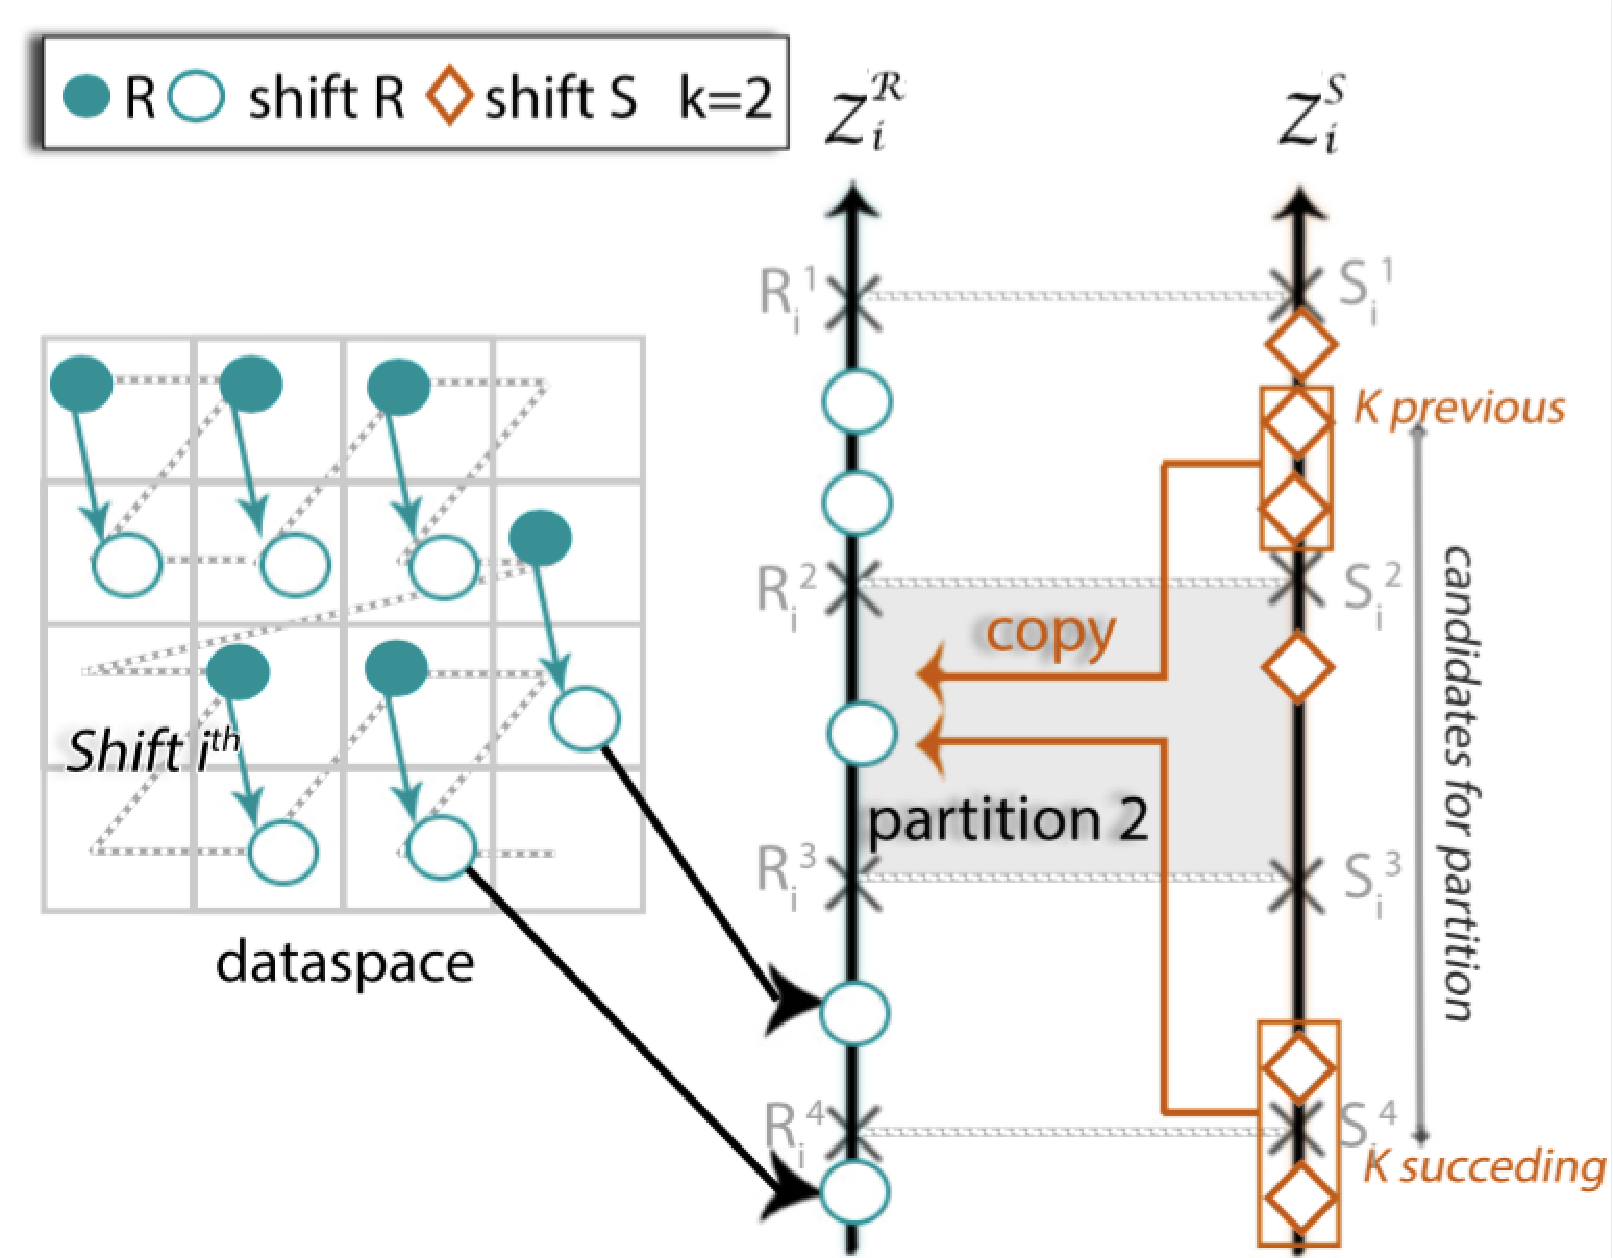
\includegraphics[width=\textwidth]{res/projection-partition.pdf}
%\caption{$z$-value : partition}
% \label{projection_partition_figure}
%\end{subfigure}%
%        \begin{subfigure}[b]{0.33\textwidth}
%                 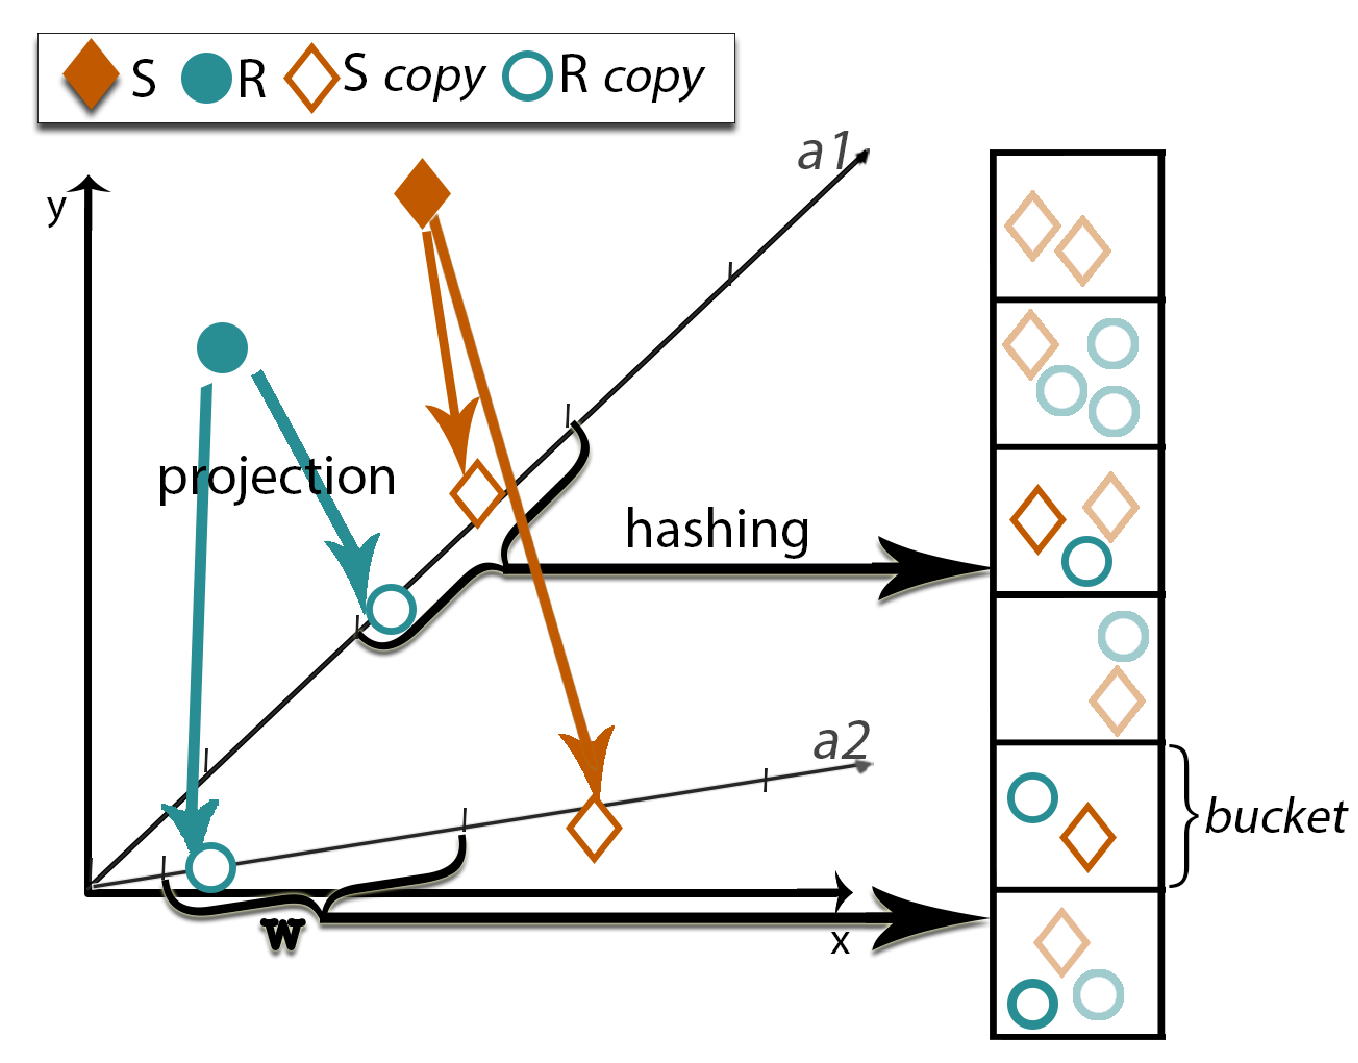
\includegraphics[width=\textwidth]{res/lsh-partition.pdf} 
%                \caption{LSH : bucket %based partitioning
%                 }
%                \label{lsh_partition_figure}
%        \end{subfigure}%
%        \begin{subfigure}[b]{0.33\textwidth}
%                 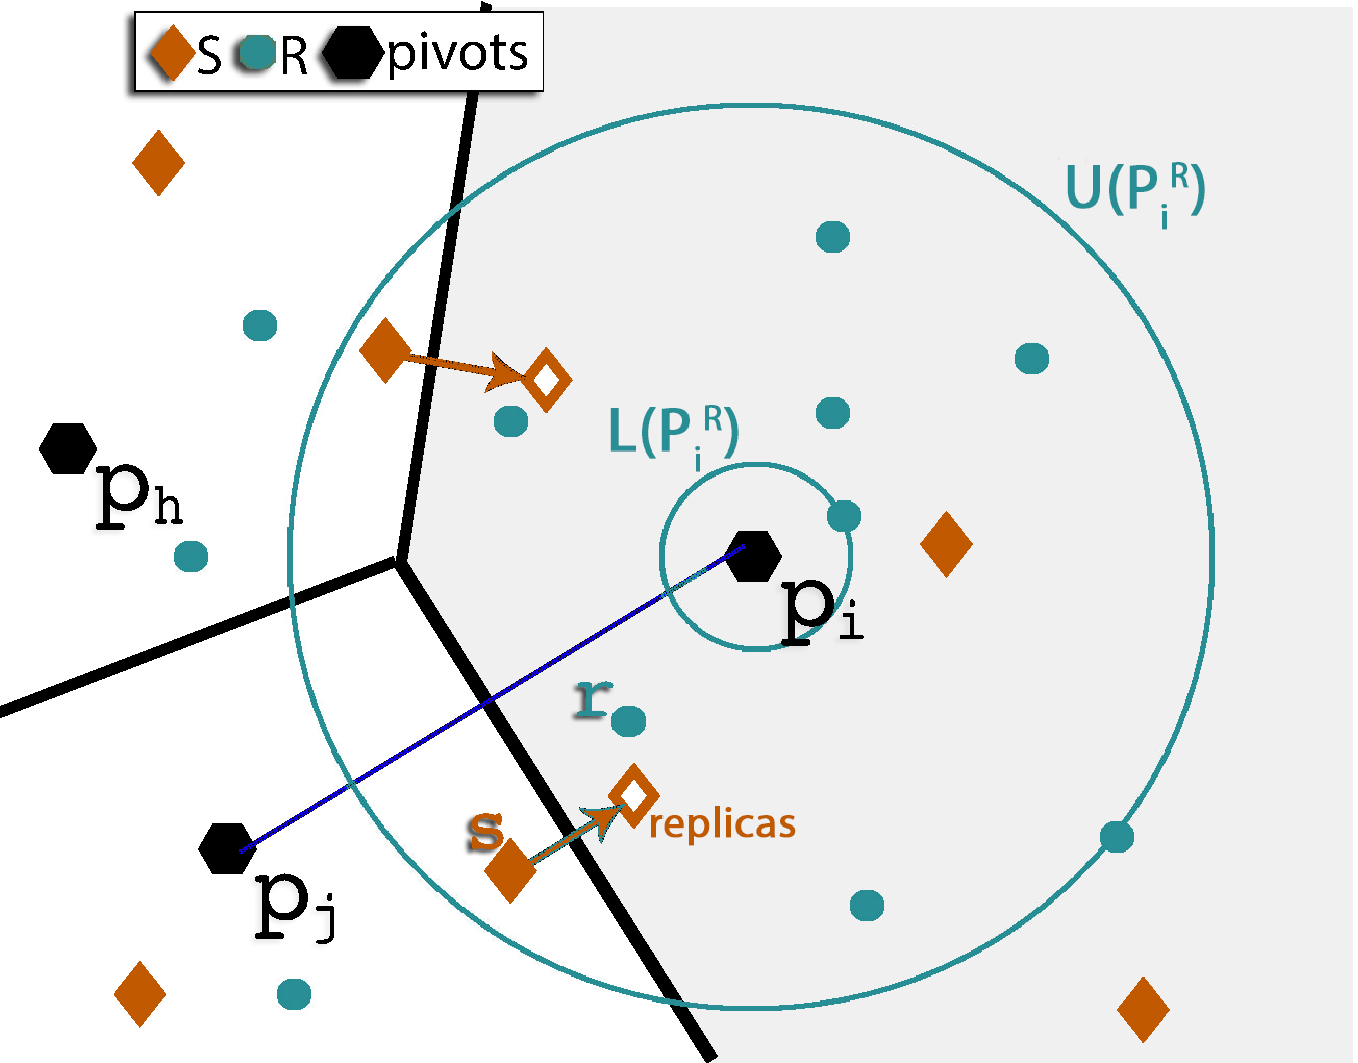
\includegraphics[width=\textwidth]{res/voronoi-partition.pdf} 
%                \caption{Voronoi : cells %based partitioning %for pivots $P_i$ and $P_j$
%                }
%                \label{fig:voronoi_partition_figure}         
%        \end{subfigure}%
% \caption{ Different partitioning and replication methods }
% \label{fig:geo_impact_k}
%\end{figure*}

\subsection{Data Partitioning and Selection}
\label{partitioning}
%kNN join is one type of spatial joins. It is a computation-intensive operation, because we should compute the pairwise 
%distance for every elements in R 
%and in S. So parallel processing is a good way for this operation especially when the size and dimension of data are big. 
%\TODO{we start directly with mapreduce, why not with centralized approaches? -- Discussion Needed --}
MapReduce is a shared-nothing platform, so in order to process data on MapReduce, we need to divide the dataset into independent pieces, 
called partitions. When computing a kNN, we need to divide $R$ and $S$ respectively.
%It is also possible to use efficient data structures such as $B^{+}-Tree$ \cite{DBLP:journals/tods/JagadishOTYZ05} and $R-Tree$ \cite{MuX} to improve local searching inside a partition.
As in any MapReduce computation, the data partition strategy will strongly impact CPU, network communication and disk usages, which in turn will impact the overall processing time \cite{DBLP:conf/hpcc/SongMHMYL13}. Besides, a good partition strategy could help to reduce the number of data replications, thereby reducing the number of distances needed to be calculated and sorted.

However, not all the algorithms apply a special data partition strategy. For example, H-BNLJ simply divides $R$ into rows and $S$ into lines, making each subset of $R$ meeting with every subset of $S$. This ensures the distance between each object $r_i$ in $R$ and each object $s_j$ in $S$ will be calculated. This way of dividing datasets causes a lot of data replications. For example, in H-BNLJ, each piece of data is duplicated $n$ times (n is the number of subsets of $R$ and $S$), resulting in a total of $n^2$ tasks to calculate pairwise distances. This method wastes a lot of hardware resources, and ultimately leads a low  efficiency.

The key to improve the performance is to preserve spatial locality of objects when decomposing data for tasks \cite{Zhou:1998:DPP:594718.594759}. This means making a coarse clustering in order to produce a reduced set of neighbors that are candidates for the final result. Intuitively, the goal is to have a partitioning of data such that an element in a partition of $R$ will have its nearest neighbors in only one partition of $S$. 
%More precisely, what we want is:
%for every partition $R_i$ ($\cup_{i}R_i=R$), find a corresponding partition $S_j$ ($\cup_{j}S_j=S$), where:
%\begin{center}
%$kNN(R_i \ltimes S) = kNN(R_i \ltimes S_j)$, and, 
%$kNN(R \ltimes S) = \bigcup kNN(R_i \ltimes S_j)$
%\end{center}
%which means that, not only it is possible to compute kNN for each element of $R_i$ in a single $S_j$, but also the concatenation of the results for all $R_i$ is equal to the global kNN join.
Two partitioning strategies that enable to separate the datasets into independent partitions, while preserving locality 
information, have 
been proposed. They are described in the two next sections. 

\subsubsection{Distance Based Partitioning Strategy}
The distance based partitioning strategy we study in this paper is based on Voronoi diagram, a method to divide the space into disjoint cells. We can find other distance-based partitioning methods in the litterature, such as in~\cite{Ji:2012:IGK:2408853.2408998}, but we chose Voronoi diagram to represent distance-based partitioning method because it it can apply to data in any dimension. 
The main property of Voronoi diagram 
is that every point in a cell is
closer to the pivot of this cell than to any other pivot. More formally, the 
definition of a Voronoi cell is as follow:
\begin{myDef}
Given a set of disjoint pivots: \\ P = $\left\{ p_1, p_2, ..., p_i, ..., p_n \right\}$, the Voronoi Cell of $p_i$ $\left(0 < 
i \leq n \right)$ is: $
\forall$ i $\neq$ j, $VC\left(p_i\right) = \left\{p \| d\left(p, p_i\right) \leq d\left(p, p_j\right) \right\}$. 
\end{myDef}


Paper \cite{Lu:2012:EPK:2336664.2336674} gives a method to partition  datasets $R$ and $S$ using Voronoi diagram. 
The partitioning principles are illustrated in Figure~\ref{fig:voronoi_partition_figure}. 
\begin{figure}[h]
\centering
\scalebox{0.33}{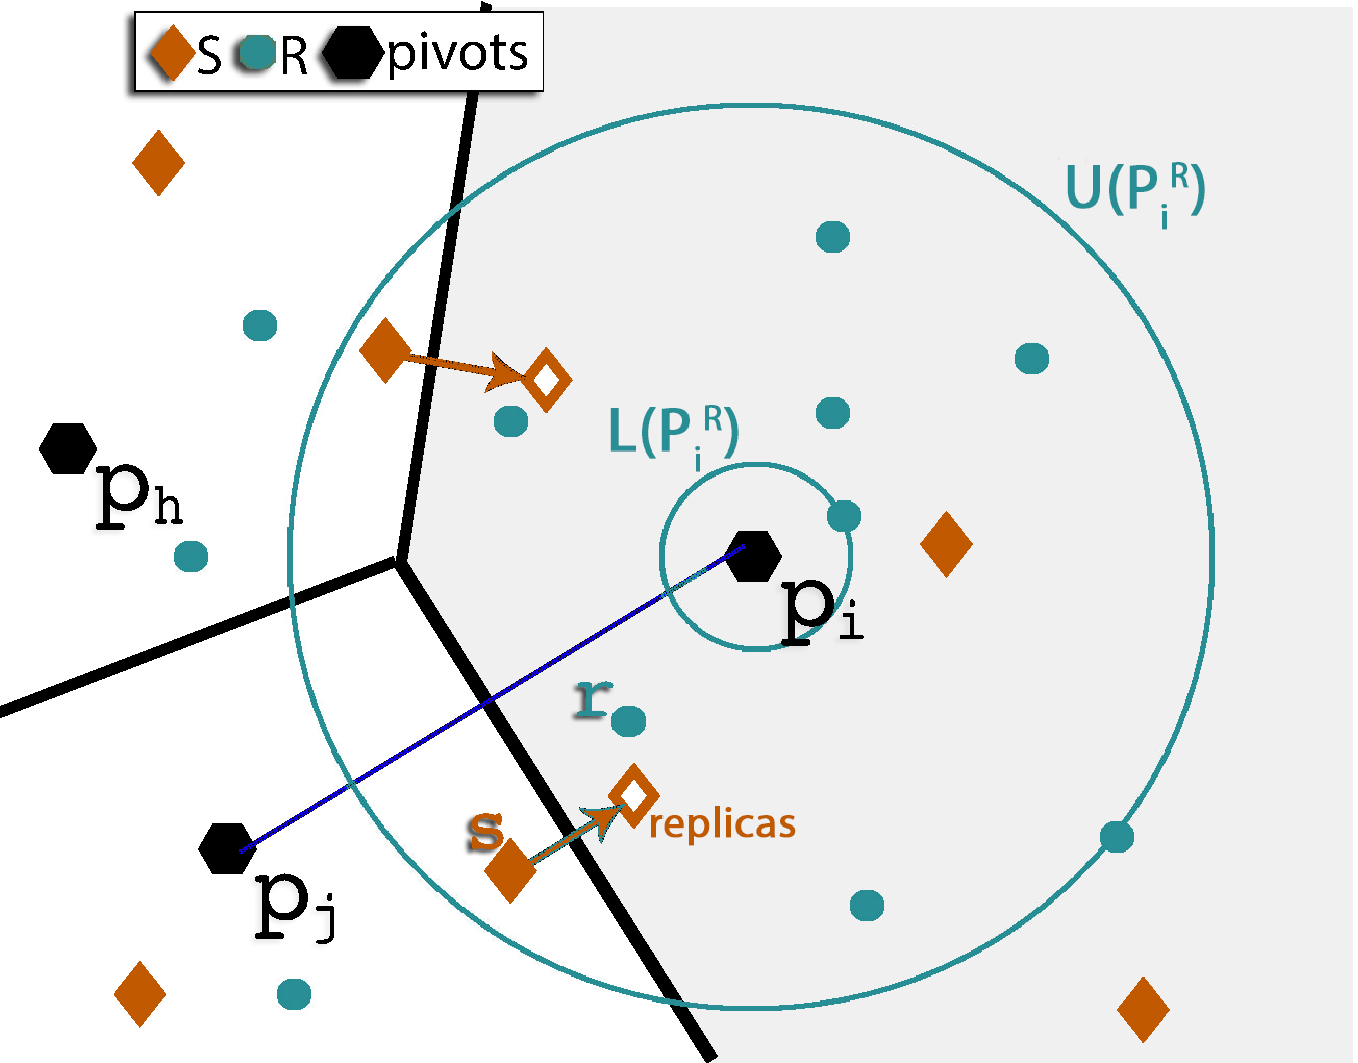
\includegraphics[width=\textwidth]{res/voronoi-partition.pdf} }
                \caption{Voronoi : cells partitioning and replication for cell $P_i$%based partitioning %for pivots $P_i$ and $P_j$
                }
                \label{fig:voronoi_partition_figure}         
\end{figure}%
After having identified the pivots $p_i$ in $R$ (c.f. Section~ \ref{data_preprocessing}), the distances between 
elements of each dataset and the pivots are computed. The elements are then put in the cell of the closest 
pivot, giving a partitioning of $R$ (resp. $S$) into $P_i^R$ (resp. $P_i^S$). For each cell, the upper bound 
$U(P^{R}_{i})$ (resp. the lower bound $L(P^{R}_{i})$) is computed as a sphere determined by the furthest (resp. 
nearest) point in $P_i^R$ from the pivot $p_i$.  The boundaries and other statistics are used to find 
candidate data from S in the neighboring cells. These data are then replicated in cell $P_i^S$. For example, in 
Figure~\ref{fig:voronoi_partition_figure}, the element $s$ of $P^{S}_{j}$ falls inside $U(P^{R}_{i})$ and is thus 
copied to $S_i$ as a potential candidate for the kNN of $r$.% \TODO{Check paper}. 



The main issue with this method is that it requires computing the distance from all elements to the pivots. Also, the distribution of the input data might 
not be known in advance. Hence, pivots have to be recomputed if data change.
 More importantly, there is no 
guarantee that all cells have an equal number of elements because of potential data skew. This can have a negative impact on the overall performance
because of load balancing issues. To alleviate this issue, the authors propose two grouping strategies, which will be discussed in 
Section~\ref{sec:load_balance}.

\subsubsection{Size Based Partitioning Strategy} 

Another type of partitioning strategy aims at dividing data into equal size partitions. Paper \cite{Zhang:2012:EPK:2247596.2247602} proposes a partitioning strategy based on $z$-value described in the 
previous section. 
%They first compute the $z$-value of every points in $R$.

%In order to have a similar number of elements in all $n$ partitions, the authors first sample the dataset and compute the the $n$ quantiles. These quantiles are an  unbiased estimation of the bounds of each partition. Figure~\ref{projection_partition_figure} shows the partition bounds arising from the $z$-value method, and highlights $i$, a shifted data.
In order to have a similar number of elements in all $n$ partitions, the authors first sample the dataset and compute the $n$ quantiles. These quantiles are an  unbiased estimation of the bounds for each partition. Figure~\ref{projection_partition_figure} shows an example for this method. In this example data are only shifted once. Then, data are projected using $z$-value method, and the interpolating ``Z" in the figure indicates the neighborhood after projection. Data is projected into a one dimension space, represented by 
$Z_{i}^{R}$ and $Z_{i}^{S}$ in the figure. $Z_{i}^{R}$ is divided into partitions using the sampling estimation explained above. For a given partition $R_i$, its corresponding $S_i$ is defined in $Z_{i}^{S}$ by copying the nearest $k$ preceding and the nearest $k$ succeeding points to the boundaries of $S_i$.
In  Figure~\ref{projection_partition_figure}, four points of $S_i$ are copied in partition 2, because they are considered as candidates for the query points in $R_i^2$.
%As said before, data are shifted in order to increase the result accuracy. After the shifted data being projected with the $z$-value space filling curve method (the 'Z' are visible thanks to the dotted line on Figure~\ref{projection_partition_figure}), data can be ordered in a dataspace of one dimension, represented on Figure~\ref{projection_partition_figure} by dataspace lines $Z_{i}^{R}$ and $Z_{i}^{S}$. Thanks to the previous sampling estimation, the dataspace lines can be divided into partitions.
%For a given partition of $R_i$, its $kNN$ candidates from $S_i$ are looked up in the dataspace line $Z_{i}^{S}$. For this, the $k^th$ preceding and the $k^th$ succeeding points of $S_i$ are copied in in the bounds of the given partition of $R_i$. For example on Figure~\ref{projection_partition_figure}, four points of $S_i$ are copied in partition 2, because they are considered as candidates for the $k$NN of the points of $R_i$ in partition 2.

%\TODOREP{First of all, In the goal of increasing of accuracy, Z-Value creates some shifts of data(here i). Then it projects the data shifted i thanks to space filling curve method, the Z dotted. So, it obtains a map of data for each shift $i$, represented here by the 2 line $Z_{i}^{R}$ and $Z_{i}^{S}$ . Thanks to sampling estimation,  it cuts the maps in partition. For a partition of $R_i$, for example here the number 2, it searches the candidates $S_i$ in the map  $Z_{i}^{S}$. For this, It copies the k preceding and the k succeeding of the boundaries of the partition 2. I considers them and the partition 2 of $S_i$  like candidates for $knn$ of the partition 2. \sout{It apply a Btree above to get the right knn.} }
 
\begin{figure}[h]
\centering
\scalebox{0.3}{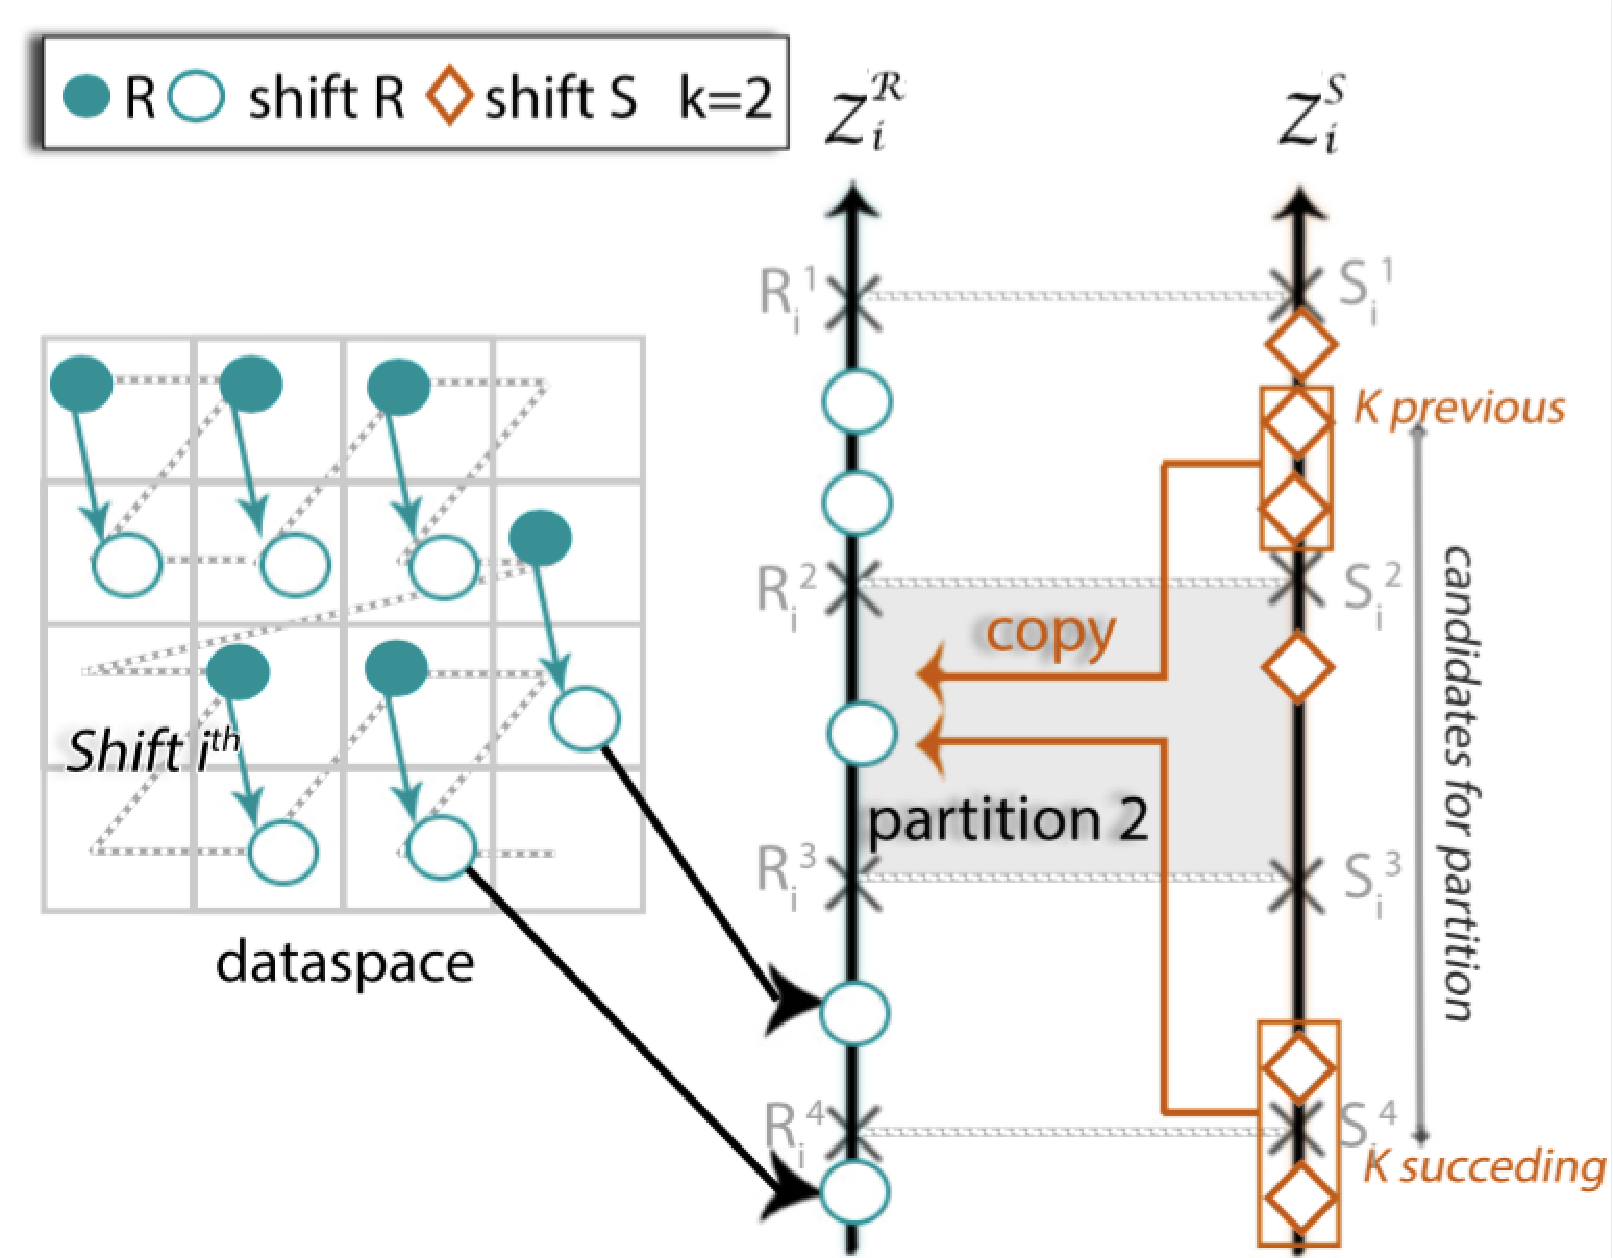
\includegraphics{res/projection-partition.pdf}}
\caption{$z$-value : partition \label{projection_partition_figure}}
%\TODOREP{Je n'aime pas cette figure ! ca fait depuis novembe que je le dit}
%}
\end{figure}


This method is likely to produce a substantially equivalent number of objects in each partition, thus naturally 
achieving load balancing. However, the quality of the result depends solely on the quality of the $z$-curve, which 
might be an issue for high dimension data. 


 
Another similar size based partitioning method uses Locality Sensitive Hashing to first project data into low dimension 
space as illustrated in Figure~\ref{lsh_partition_figure}. In this example, data is hashed twice using two hash 
families $a1$ and $a2$. Each hashed data is then projected in the corresponding bucket. The principle of this method is 
to result in collisions for data that is spatially close. So the data initially close in the high dimension space is 
hashed to the same bucket with a high probability, provided that the bucket size (parameter $W$ in LSH) is large enough 
to receive at least one copy of close data. 

 
The strategy of partitioning directly impacts on the number of tasks and the amount of computation. Distance based 
methods aim at dividing the space into cells that are driven by distance rules. Size based methods create equal size 
zones in which the points are ordered.
Regarding the implementation, \cite{Lu:2012:EPK:2336664.2336674} uses a MapReduce job to 
perform the partitioning. In \cite{Zhang:2012:EPK:2247596.2247602}, both data preprocessing and data partitioning are completed in a single MapReduce job.

\begin{figure}[h]
\centering
\scalebox{0.33}{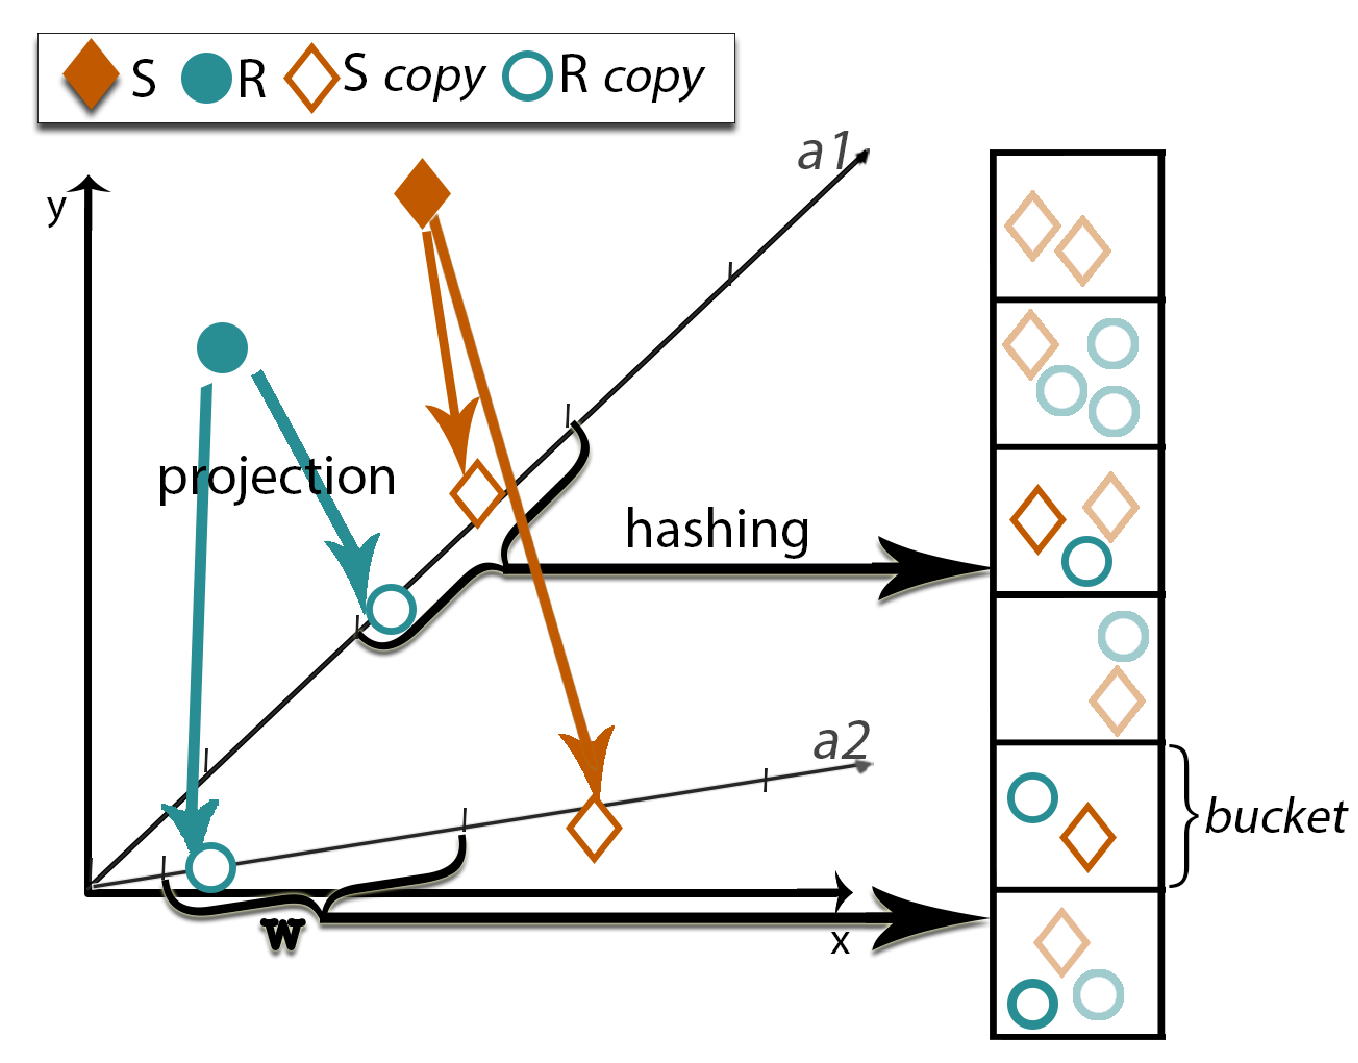
\includegraphics{res/lsh-partition.pdf}}
\caption{LSH : bucket \label{lsh_partition_figure}}
\end{figure}
%LSH is an approximate approach and }. 
%Although it's more probable for the related objects to have the same hash value than the distance ones, normally one hash function can not guarantee
%the accuracy. We often need a group of hash functions to generate multiple hash tables to avoid the conflict probability of close objects.  
